The Economic Research Service (ERS), an agency under the U.S. Department of Agriculture for which commuting zones were originally developed, distributes definitions on its website.\footnote{ERS has released commuting zone definitions based on 1980, 1990, and 2000 commuting data. All three definitions are available at http://www.ers.usda.gov/data-products/commuting-zones-and-labor-market-areas.aspx.} Commuting Zones are especially relevant for the economic analysis of rural areas, a focus of ERS, because they include all counties, not just urban counties.

As an alternative to metropolitan statistical areas, or Core Based Statistical Areas \citep{OMB2013}, many researchers examining local labor markets use commuting zones, which also combine sets of counties based on commuting flows, because they cover the entire country. However, few researchers are familiar with the methodology used to develop these zones. To that end, this section describes the methodology used by \cite{TS1996} in developing the zones.\footnote{The methodology was originally used in \cite{TK1987}, but the 1996 paper is much more
widely cited, and the zones from that paper are the ones most commonly used. For more background on the development of commuting zones, see \cite{FowlerRhubartJensen2016}.}

We describe two especially important design components: the dissimilarity matrix, which measures how ``far'' nodes are from one another, and the clustering method, which decides how nodes are assigned to groups.

\subsection{Dissimilarity Matrix}

The dissimilarity matrix, $D$, is a representation of the relative distance between all pairs of counties. TS calculate $D$ (or conversely, the similarity matrix $P$), where an entry $D_{ij}$ is the dissimilarity of county $i$ from county $j$, as below:\footnote{The clustering method used requires a dissimilarity matrix; one is just the complement of the other, by element, so $D_{ij}=(1-P_{ij})$.}

\begin{equation}\label{eqn:diss}
D_{ij} = 1- \frac{f_{ij}+f_{ji}}{\min(rlf_{i},rlf_j)}
\end{equation}

In the above equation, $f_{ij}$ is the flow of commuters who live in county $i$ and work in county $j$ and $f_{ji}$ is the opposite flow. The resident labor force in county $i$ is $rlf_i = \sum_j f_{ij}$ (including $f_{ii}$), with a similar calculation for $j$. Normalizing flows with the minimum resident labor force of a pair upweights the association of outlying areas with metropolitan cores. Note that disimilarity is symmetric, so $D_{ij}=D_{ji}$.

TS1996 compute $D$ using flows from the 1990 Journey-to-Work data, which tabulates the commuting information from the 1990 Census Long-form \citep{Census1990jtw}.\footnote{Journey to Work data on county to county commuting flows are available for the 1990 Census, the 2000 Census, and 5-year samples of the American Community Survey at \url{https://www.census.gov/hhes/commuting/data/commutingflows.html}.} The Census Bureau estimates county-to-county flows among 3,141 county equivalents for persons age 16 and older who reported being employed in the week prior to April 1, 1990.\footnote{Employment status is based on responses to the question ``Did this person work at any time LAST WEEK?'' Place of work is geocoded using the response to ``At what location did this person work LAST WEEK?'' Residence location is compiled from the mailing frame of the Census.} The Economic Research Service maintains the 1990 commuting zones.%
% This is a repeat from further up
%\footnote{Other releases of commuting zones have used 1980 and 2000 data. All three are available at \url{http://www.ers.usda.gov/data-products/commuting-zones-and-labor-market-areas.aspx}.} 

\subsection{Clustering Method}

After constructing this dissimilarity matrix, TS use it as an input into their clustering method. In general, data scientistcs use clustering methods to assign interrelated items, or items with similar features, into groups. In their application, TS use the average-linkage hierarchical clustering algorithm (PROC CLUSTER in SAS software).\footnote{The hierarchical clustering for this paper using PROC CLUSTER was generated using SAS software, Version 9.2 of the SAS System for Unix. Copyright \copyright 2009 SAS Institute Inc. SAS and all other SAS Institute Inc. product or service names are registered trademarks or trademarks of SAS Institute Inc., Cary, NC, USA.}
The hierarchical clustering method uses the dissimilarity matrix in the following way. To begin, every county is its own cluster. Then, it finds the lowest value $D_{ij}$ in the dissimilarity matrix, and combines those two counties together. It then recalculates the dissimilarity values between the new cluster and all other clusters. For each pair of clusters $C_K$ and $C_L$, the dissimilarity, $D_{KL}$, is calculated as:

\begin{equation}
D_{KL} = \frac{1}{N_K N_L} \sum_{i \in C_k} \sum_{j \in C_L} D_{ij},
\end{equation}

where and $D_{ij}$ is calculated as in Equation \ref{eqn:diss} and $N_K$ and $N_L$ are the count of nodes, or counties in this case, in each cluster. The process continues until all nodes are clustered, though the designer may stop the process by choosing a maximum ``cutoff'' height, $H$, such that if $D_{KL}>H$, then $K$ and $L$ do not merge. TS1990 uses clusters with distances up to $0.98$.

We illustrate this process in Appendix Figure \ref{fig:caliclusters}, which shows the hierarchical progression of how counties are clustered together for California. In the top left-hand corner, only a few counties have joined at a height of $H=0.80$. As we increase the height to 0.88 and to 0.96, more counties are joined together. Finally, at a height of 1, almost all the counties have merged together, forming one large cluster and a few much smaller clusters.

\subsection{Our Replication}
\FloatBarrier

In order to replicate the clustering result in TS, which we refer to as TS1990, we use the 1990 Census JTW data and the methodology described above, with one important exception. Because of computing power constraints in 1996, TS divided the country into six overlapping regions and performed the clustering algorithm on each region separately, and then manually resolved conflicts in overlapping regions. This decision has two consequences for users: first, the height cutoffs across regions are not the same, because there is a normalization step before the algorithm merges observations. Second, it induces some subjectivity, since conflicts in cluster assignment for counties in the overlapping regions are inevitable.

Rather than follow their methodology and divide the country into regions, we run the hierarchical clustering algorithm on the entire country, and use the height cutoff that most closely replicates their original count of zones, which we find to be 0.9418. TS1996's zones and our replication are in Figure \ref{fig:czreplication}, and our summary statistics comparing the zones are in Table \ref{tab:replication}. Our replication has more evenly sized clusters with fewer clusters made up of a single county. We refer to our replication as FKV1990.

While our replication does not perfectly match their zones and the cutoff height differs, this is not surprising, because we did not split the country into overlapping regions. With that caveat, our replication matches the moments from the commuting zones closely, and for a given county, about 80\% of the counties in our new zones match with the counties in the original zones.
\begin{figure}[tbh]\centering
\begin{tabular}{cc}
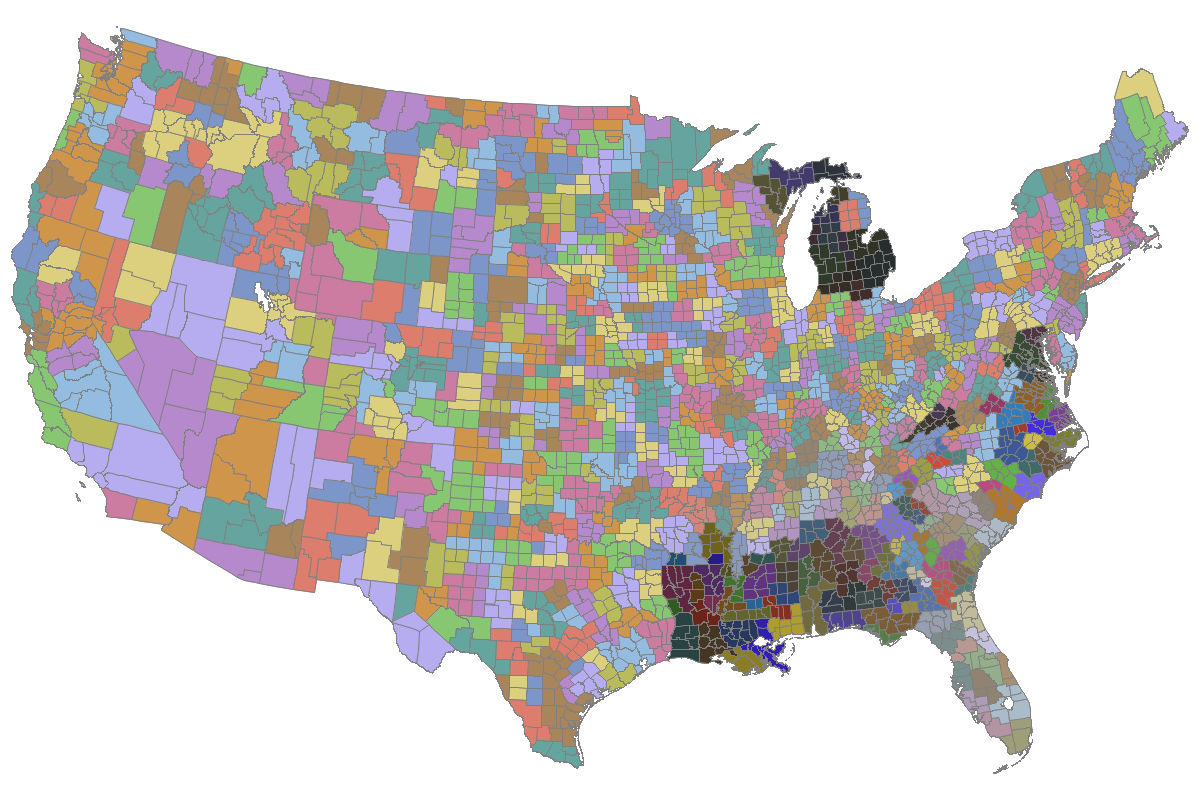
\includegraphics[scale=0.25]{./figures/commutingzones.png}&
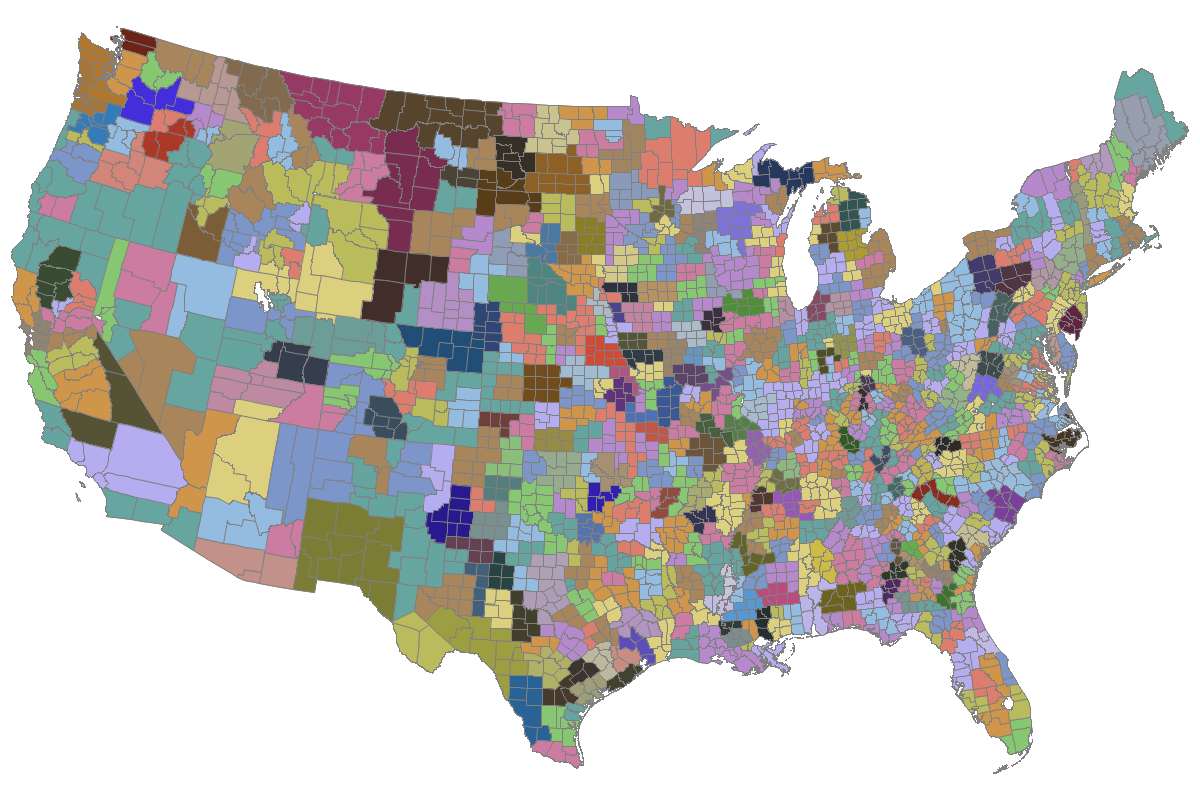
\includegraphics[scale=0.25]{./figures/clustermap_jtw1990_x.png}\\
Commuting Zones - TS1990 & Replication of Commuting Zones - FKV1990 \\
\end{tabular}
\caption{Replication of Commuting Zones from TS1996: County Mapping \label{fig:czreplication}}
\end{figure}

% source: name of SAS program
% Last updated:

\begin{table}\centering
\caption{Replication of Commuting Zones from TS1996: Summary Statistics \label{tab:replication}}
\begin{tabular}{lcc}
\hline\hline
       & TS1990 &  FKV1990  \\
       \hline
Mean Cluster Size &  4.24  & 4.19 \\
Median Cluster Size & 4 & 4 \\
Number of Clusters & 741 & 741  \\
Number of Singletons & 62 &  10 \\
\hline
\multicolumn{3}{p{4in}}{\footnotesize \textit{Notes}: Both TS1990 and FKV1990 are based on JTW tabulations from the 1990 Census. Summary statistics for TS1990 are from Table 8 of TS1996.}\\
\end{tabular}
\end{table}


%Mark will look at writing a more efficient macro for this
